% !TeX root = ../main.tex

\chapter{地面运行的LXeTPC本底研究}
\label{sec:backgrounds}

为了定量地描述实验对某些物理参数的灵敏度,我们需要对实验本底进行估计。
本章使用蒙特卡洛方法(Monte Carlo method)估计两类实验中的主要本底:$\mu$子本底和材料放射性本底。

\section{模拟框架}

Geant4 是辐射探测和粒子物理领域常用的以C++为基础的蒙特卡洛模拟软件包\cite{agostinelli_geant4simulation_2003,allison_geant4_2006,allison_recent_2016}。
PandaX合作组基于Geant4开发了BambooMC软件包用于PandaX实验中的探测器模拟\cite{chen_bamboomc_2021}。
BambooMC具有较强的可拓展性,本文中使用基于BambooMC开发的软件包RelicsSim对地表附近探测器$\mu$事件和材料本底进行模拟。
所用几何如图\ref{fig:relics_g4}所示,结构遵循\ref{fig:relics_geo}的设计。

\begin{figure}
  \begin{subfigure}{.5\textwidth}
    \centering
    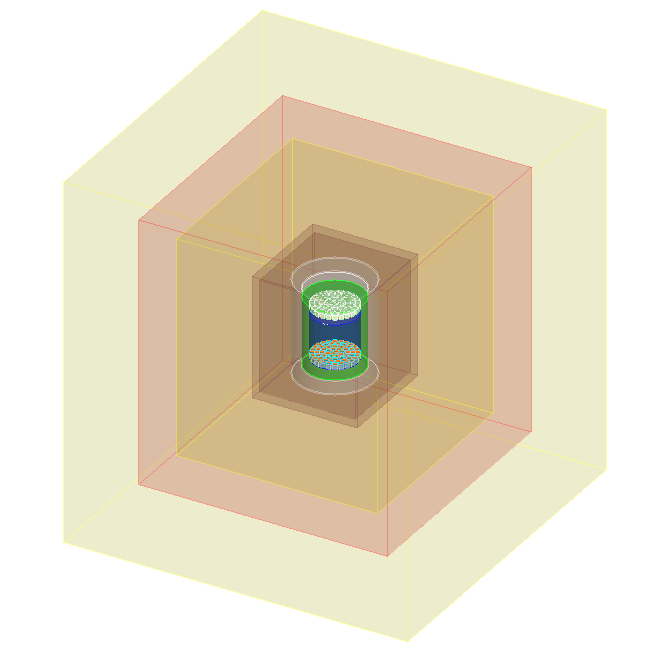
\includegraphics[width=1.0\linewidth]{figures/relics_outer.png}
    \caption{\label{fig:relics_outer} LXeTPC屏蔽体几何}
  \end{subfigure}
  \begin{subfigure}{.5\textwidth}
    \centering
    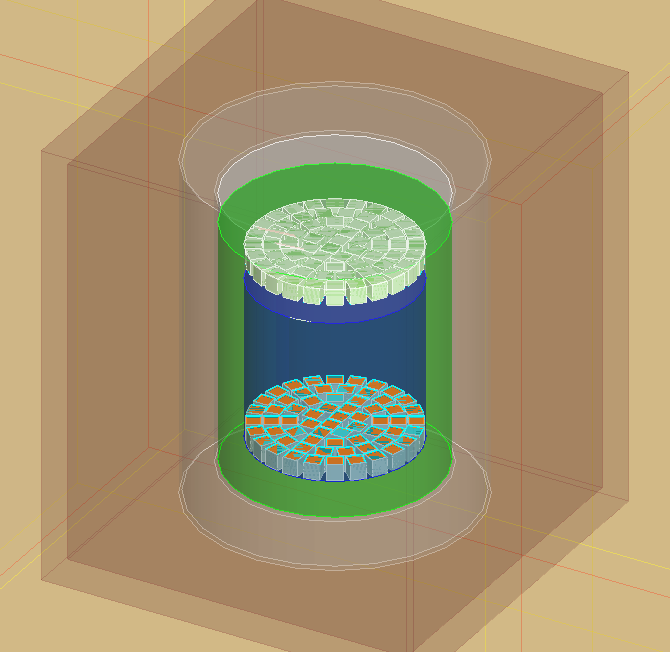
\includegraphics[width=1.0\linewidth]{figures/relics_inner.png}
    \caption{\label{fig:relics_inner} LXeTPC中心探测器几何}
  \end{subfigure}
  \caption{\label{fig:relics_g4} RelicsSim中屏蔽体和探测器几何探测器,绿色体积为液氙4$\pi$反符合探测器,蓝色体积为中心主探测器。}
\end{figure}

探测器基本参数列在表\ref{tab:relics_material}中。

\begin{table}
  \centering
  \caption{LXeTPC几何参数}
  \begin{tabular}{cccc}
    \toprule
    名称 & 几何体 & 参数 & 材料 \\
    \midrule
    外聚乙烯屏蔽体 & 空心长方体 & $216\times216\times226\si{cm^3}$ & 高密度聚乙烯 \\
    铅屏蔽体 & 空心长方体 & $156\times156\times166\si{cm^3}$ & 铅 \\
    内聚乙烯屏蔽体 & 空心长方体 & $126\times126\times136\si{cm^3}$ & 高密度聚乙烯 \\
    铜屏蔽体 & 空心长方体 & $66\times66\times76\si{cm^3}$ & 铅 \\
    空气层 & 空心长方体 & $60\times60\times70\si{cm^3}$ & 空气 \\
    外不锈钢罐体 & 空心圆柱体 & 厚度$0.5\si{cm}$,高$59\si{cm}$,直径$48\si{cm}$ & 不锈钢 \\
    真空隔热层 & 空心圆柱体 & 厚度$5\si{cm}$,高$58\si{cm}$,直径$47\si{cm}$ & 真空 \\
    内不锈钢罐体 & 空心圆柱体 & 厚度$0.5\si{cm}$,高$58\si{cm}$,直径$37\si{cm}$ & 不锈钢 \\
    外层气态氙 & 圆柱体 & 高$5\si{cm}$,直径$36\si{cm}$ & 气态氙 \\
    液氙反符合层 & 空心圆柱体 & 厚度$4\si{cm}$,高$42\si{cm}$,直径$36\si{cm}$ & 液态氙 \\
    内层气态氙 & 圆柱体 & 高$6\si{cm}$,直径$28\si{cm}$ & 气态氙 \\
    液氙主探测器 & 圆柱体 & 高$28\si{cm}$,直径$28\si{cm}$ & 液态氙 \\
    \bottomrule
  \end{tabular}
  \label{tab:relics_material}
\end{table}

液氙主探测器上下分别有64个1英寸光电倍增管:日本滨松R8520,共128个。光电倍增管的几何如图\ref{fig:pmt_geo}。

\begin{figure}
  \begin{subfigure}{.5\textwidth}
    \centering
    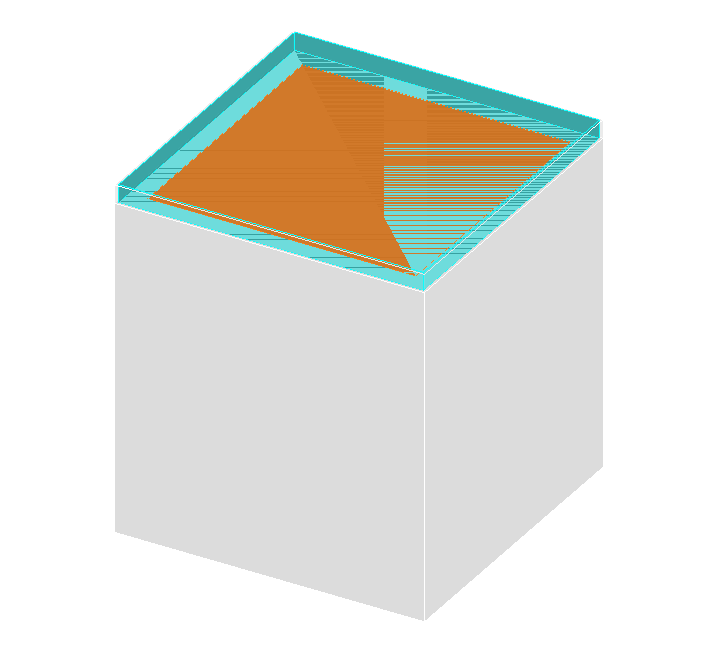
\includegraphics[width=1.0\linewidth]{figures/pmt_geo.png}
    \caption{\label{fig:pmt_g4} R8520在Geant4中的几何}
  \end{subfigure}
  \begin{subfigure}{.5\textwidth}
    \centering
    \includesvg[width=1.0\linewidth]{figures/topPMTs.svg}
    \caption{\label{fig:pmt_layout} PMT在探测器$(x,y)$平面上的排布}
  \end{subfigure}
  \caption{\label{fig:pmt_geo} 光电倍增管R8520的几何和在探测器$(x,y)$平面上的排布。
  蓝色透明几何为石英窗;橙色几何为光阴极(photocathode);灰色部分是套管(casing),材质为SAE 304不锈钢。
  排布保证了轴向对称性,可能对未来的位置重建有利。}
\end{figure}

PMT石英窗上富集的${}^{40}\mathrm{K}$和${}^{137}\mathrm{Cs}$可能成为主要的本底来源,具体内容将在第\ref{sec:pmt_background}章中讨论。

\section{本底事件的筛选与压低}

本底事件经常与信号有不同的性质以及测量结果。
对于$\mu$子本底,其可能强烈地在液氙反符合层中沉积能量,可以用反符合层对$\mu$子的标记将其本底压低。
同时$\mu$子将可能在主探测器中多次沉积能量
材料的$\beta$和$\gamma$放射性在中心探测器边缘单位体积沉积的能量比探测器中心多,所以一定程度地舍弃某些本底过高的区域,
对物理信号的搜索是有利的。

\section{$\mu$子本底}

地面附近运行的LXeTPC将会经受原生宇宙线和次生宇宙线的轰击。
来自外部空间的宇宙线成分以高能质子为主,在穿越地球大气层的过程中与大气分子发生簇射反应,产生大量次级粒子,
主要包括质子、$\mu$子、电子、中子、$\gamma$光子等。宇宙线粒子通量与大气层深度有关,如图\ref{fig:vertical_flux}。

\begin{figure}
    \centering
    \includesvg[width=0.7\linewidth]{figures/vertical_flux.svg}
    \caption{\label{fig:vertical_flux} 宇宙线中不同粒子通量与大气深度的关系\cite{olive_review_2016}。
    $\mu$子和中微子是地面附近通量最高的两种粒子,中微子较少与物质发生相互作用,$\mu$子成为实验中的主要本底。}
\end{figure}

$\mu$子是带电粒子,穿透能力较强。$\mu$子穿越物质的过程中通过电磁相互作用减速,产生电离,
高能($10\si{GeV}$以上)$\mu$子在物质中的能损$-\mathrm{d}E/\mathrm{d}x$大约为$2\si{MeV\cdot cm^{-1}}$。
考虑相对论时间膨胀效应,$\mu$子在物质中能够穿越较长距离。$\mu$子还有可能被原子核俘获,
使靶原子核序数减1,同时放出1个或多个中子。这些中子将是探测器中核反冲本底的主要来源。

利用$\mu$子持续产生电离的特点,可以在探测器外围部署$\mu$子反符合探测器,
当$\mu$子同时在反符合探测器和主探测器产生信号且符合一定条件时时,通过硬件触发或软件筛选,
可以将主探测器中事件标记为$\mu$子事件以区分信号的本底。但物理信号如CE$\nu$NS也有一定几率发生在$\mu$子穿越探测器时,
这时对$\mu$子事件的标记会使物理信号的探测效率降低,等效为曝光量(exposure)的损失,这种效应必须考虑到统计推断中,
否则将高估探测器中产生的信号。

地面附近的$\mu$子分布可以用Gaisser公式或Shukla公式描述。T.K.Gaisser在忽略地球曲率的情况下,
给出了$\mu$子通量随$\mu$子能量$E_\mu$和天顶角(zenith angle)$\theta$的分布。天顶角为入射粒子与地面法线间的夹角\cite{gaisser_cosmic_2016}。

\begin{align}
    \label{eq:gaisser}
    \frac{\mathrm{d}N_\mu}{\mathrm{d}E_\mu\mathrm{d}\Omega} &\approx 
    1400E_\mu^{-2.7}/\left(\si{m^2\cdot s\cdot GeV\cdot sr}\right)\left(\frac{1}{1+\frac{1.1E_\mu\cos\theta}{\epsilon_\pi}}+\frac{0.054}{1+\frac{1.1E_\mu\cos\theta}{\epsilon_\kappa}}\right)
\end{align}

其中$\epsilon_\pi\approx115\si{GeV},\epsilon_\kappa\approx850\si{GeV}$。
Gaisser公式只在高能区间($E_\mu>(100/\cos\theta)\si{GeV}$)适用。

P.Shukla等人在考虑地球曲率的条件下给出了类似的分布\cite{shukla_energy_2018},如式\ref{eq:shukla}:

\begin{align}
    \label{eq:shukla}
    I\left(E_\mu,\theta\right) &= I_0 N\left(E_0+E_\nu\right)^{-n}\left(1 + \frac{E_\mu}{\epsilon_\mu}\right)^{-1}D(\theta)^{-(n-1)} \\
    D(\theta) &= \sqrt{\frac{R^2}{d^2}\cos^2\theta+2\frac{R}{d}+1}-\frac{R}{d}\cos\theta
\end{align}

其中$I_0$为绝对流强,$N$为归一化参数,$n$为天顶角分布的幂次,$\epsilon_\mu,\frac{R}{d}$为经验公式中的自由参数。
使用不同地点测量得到的$\mu$子分布可以拟合得到不同结果,这里我们使用Shukla通过日本筑波市附近的测量数据得到的拟合结果,具体参数见表\ref{tab:shukla}。
Shukla公式在低能区域和高能区域都与数据符合得较好。

\begin{table}
  \centering
  \caption{描述$\mu$子分布的Shukla公式采用的参数列表}
  \begin{tabular}{cc}
    \toprule
    符号 & 取值 \\
    \midrule
    $I_0$ & $70.7\si{m^{-2}\cdot s^{-1}\cdot sr^{-1}}$ \\
    $n$ & 3.01 \\
    $E_0$ & $4.19\si{GeV}$ \\
    $\epsilon_\mu$ & $854\si{GeV}$ \\
    $R/d$ & $174$ \\
    \bottomrule
  \end{tabular}
  \label{tab:shukla}
\end{table}

式\ref{eq:shukla}中天顶角$\theta$相关的项可以从$E_\mu$中解耦合,$\theta$和$E_\mu$的分布如图\ref{fig:shukla_distribution}。

\begin{figure}
    \centering
    \includesvg[width=1.0\linewidth]{figures/shukla_distribution.svg}
    \caption{\label{fig:shukla_distribution} Shukla公式中$\theta$和$E_\mu$的分布,$\theta$主要集中在夹角较小的区域,
    因为天顶角更大的$\mu$子与大气层中物质的相互作用路程更长,损失更多;$E_\mu$主要集中在低能部分。}
\end{figure}

到达地面附近的$\mu$子包含了$\mu^-$和$\mu^+$。
CMS于2010年测量得到了地表附近的$\mu$子电荷比(charge ratio, $I_{\mu^+}/I_{\mu^-}$)约为$1.2766\pm0.0045$\cite{the_cms_collaboration_measurement_2010}。
$\mu$子电荷比在$\mu$子动量小于$100\si{GeV/c}$时与能量几乎无关,且在更高动量的区域略增大。
考虑到第\ref{sec:muon_nr}节中讨论的$\mu$子核反冲本底主要由较低能量的$\mu^-$贡献,更高的电荷比意味着更低的核反冲本底,本文保守地使用不随能量变化的电荷比。

\subsection{核反冲本底}
\label{sec:muon_nr}

$\mu$子通过两种方式

\subsection{电子反冲本底}

\section{材料本底}

\subsection{光电倍增管本底}
\label{sec:pmt_background}

\subsection{屏蔽体材料本底}

\subsection{液氙中惰性元素本底}
